% =====================================================================
% NSEN 6684 -- Beyond the Six-Factor Formula: Neutron Leakage, Spectral
% Effects, and Reactivity Feedback in Compact Space Fission Reactors
% Author: Irais Strong, Idaho State University
%
% Compile (TeX Live or MiKTeX):  pdflatex -> bibtex -> pdflatex -> pdflatex
%   or:                          latexmk -pdf NSEN6684_Beyond_Six_Factor_Report.tex
% Figures are read from ../figures/ and code listings from ../code/.
% Numerical values are those printed in ../results/analysis_output.txt.
% =====================================================================
\documentclass[11pt,letterpaper]{article}

\usepackage[T1]{fontenc}
\usepackage[utf8]{inputenc}
\usepackage{lmodern}
\usepackage[margin=1in]{geometry}
\usepackage{microtype}
\usepackage{amsmath,amssymb}
\usepackage{siunitx}
\usepackage{booktabs}
\usepackage{tabularx}
\usepackage{graphicx}
\usepackage{float}
\usepackage[font=small,labelfont=bf]{caption}
\usepackage{xcolor}
\usepackage{listings}
\usepackage{textcomp}
\usepackage[inline]{enumitem}
\usepackage[numbers,sort&compress]{natbib}
\usepackage[hidelinks]{hyperref}

\graphicspath{{../figures/}}
\sisetup{per-mode=symbol, range-phrase=--, range-units=single}
\setlist{nosep, leftmargin=1.4em}

\definecolor{codebg}{HTML}{F6F7F9}
\definecolor{codekw}{HTML}{46607D}
\definecolor{codecm}{HTML}{6B7280}
\definecolor{codestr}{HTML}{B5523B}
\lstset{
  language=Python, basicstyle=\ttfamily\scriptsize, backgroundcolor=\color{codebg},
  keywordstyle=\color{codekw}\bfseries, commentstyle=\color{codecm}\itshape,
  stringstyle=\color{codestr}, breaklines=true, frame=single, rulecolor=\color{codecm!40},
  numbers=left, numberstyle=\tiny\color{codecm}, showstringspaces=false, columns=fullflexible
}

\newcommand{\keff}{k_\mathrm{eff}}
\newcommand{\kinf}{k_\infty}
\newcommand{\PNL}{P_\mathrm{NL}}
\newcommand{\Sig}[1]{\Sigma_\mathrm{#1}}
\newcommand{\ltr}{\lambda_\mathrm{tr}}
\newcommand{\calc}{\textsc{[calculated]}}
\newcommand{\obs}{\textsc{[observed]}}
\newcommand{\infr}{\textsc{[inferred]}}

\title{\textbf{Beyond the Six-Factor Formula: Neutron Leakage, Spectral Effects, and Reactivity Feedback in Compact Space Fission Reactors}\\[0.6em]
\large Technical Report for NSEN 6684 --- Reactor Physics}
\author{Irais Strong\\[0.2em]
\normalsize Ph.D. Program in Nuclear Engineering, Idaho State University, Pocatello, Idaho}
\date{November 2026}

\begin{document}
\maketitle
\thispagestyle{empty}

\begin{abstract}
\noindent
Classical neutron life-cycle theory, summarized by the four- and six-factor formulas, provides the conceptual foundation for criticality. This report argues that compact, fast-spectrum space reactors require more: explicit neutron transport, a leakage-centred neutron balance, reflector interactions treated through boundary conditions, and temperature-dependent reactivity. The k-eigenvalue problem is formulated from the transport equation, and the one-group diffusion approximation is derived from it together with its validity conditions. A multigroup Monte Carlo transport solver was written and verified against five exact solutions from the LA-13511 analytic benchmark set: all five reproduce $\keff = 1$ within about one standard deviation ($\sigma \approx 0.0003$). With the same published, idealized cross sections, one-group diffusion underpredicts $\keff$ by 6\% in bare and 10--12\% in reflected compact spheres and overpredicts the bare critical radius by 7.3\%. Its error falls from 9.8\% to 1.9\% as the radius grows from 1.3 to 4.6 transport mean free paths. Transport gives reflector savings of 1.0--1.4~cm, which a large-core slab formula overestimates by a factor of 2.7--3.8. A two-group analysis shows that leakage preferentially removes fast neutrons, and that one-group spectral collapse error (about 1\%) is several times smaller than diffusion error here. Published KRUSTY documentation is then used to examine reflector worth and to decompose negative feedback into fuel expansion, fuel cross-section (including Doppler), reflector and structural contributions. A first-principles expansion estimate reproduces the sign and order of magnitude of KRUSTY's fuel coefficient. All calculations use idealized benchmark constants. They are mathematical illustrations, not predictions for any real reactor.
\end{abstract}

\noindent\textbf{Keywords:} k-eigenvalue; neutron transport; diffusion theory; neutron leakage; reflector savings; spectral effects; reactivity feedback; Monte Carlo; KRUSTY; space fission power.

\vspace{0.5em}
\noindent\small\textit{Scope statement.} Public information only; no proprietary, employer-specific or confidential material. Calculated results, published experimental observations and engineering inferences are labeled \calc, \obs\ and \infr\ where they are summarized (Section~\ref{sec:findings}).\normalsize

\newpage
\tableofcontents
\listoffigures
\listoftables
\newpage

% =====================================================================
\section{Introduction}
\label{sec:intro}

The thesis of this report is:
\begin{quote}
\emph{Classical neutron life-cycle theory provides the conceptual foundation for criticality, but compact fast-spectrum space reactors require more detailed consideration of neutron transport, leakage, reflector interactions, and temperature-dependent reactivity.}
\end{quote}

Space surface power gives the question practical weight. Night at low lunar latitudes lasts roughly 14 Earth days. In January 2026 NASA and DOE announced a renewed commitment to a lunar surface reactor by 2030 \citep{NASA2026MOU}, and draft Lunar Reactor-1 requirements, as publicly reported, call for at least \SI{20}{kWe} through at least \SI{354}{h} of darkness \citep{NSE2026LR1}. Systems that can be launched are small. The KRUSTY ground test of 2018 used a highly enriched uranium (HEU) core \SI{11}{cm} in diameter and \SI{25}{cm} tall \citep{Sanchez2020Component,Poston2020Design}. In cores like this, leakage is the dominant neutron loss, reflector position is the reactivity control, and expansion of the fuel is the main feedback \citep{Poston2020Design,Poston2020Results}.

The course material on the neutron life cycle covers the six-factor formula, one-group diffusion and bare-reactor buckling, with transport and Monte Carlo introduced conceptually. This report goes beyond it in four ways:
\begin{enumerate*}[label=(\roman*)]
  \item it formulates the multiplication problem as a transport eigenvalue problem and derives diffusion from it;
  \item it quantifies, against exact solutions, how much one-group diffusion misses in compact bare and reflected systems;
  \item it isolates spectral effects of leakage with a two-group model; and
  \item it uses published KRUSTY data to separate reflector worth and feedback by component.
\end{enumerate*}
The models are deliberately idealized. They test methods against known answers and are not a design tool.

% =====================================================================
\section{The Classical Neutron Life Cycle: A Brief Review}
\label{sec:classical}

In a thermal reactor one generation is tracked from thermal absorption in fuel through fast fission, fast leakage, resonance capture during moderation, thermal leakage and thermal utilization \citep{Lamarsh2001,Duderstadt1976}:
\begin{equation}
  \keff = \eta\,\varepsilon\,p\,f\,P_\mathrm{FNL}\,P_\mathrm{TNL}.
  \label{eq:sixfactor}
\end{equation}
With assumed light-water-like factors ($\eta = 1.84$, $\varepsilon = 1.03$, $p = 0.78$, $f = 0.90$, $P_\mathrm{FNL}=0.80$, $P_\mathrm{TNL}=0.95$), 1000 absorptions in fuel lead to 1011 in the next generation, so $\keff = 1.011$ (Figure~\ref{fig:lifecycle}). Equation~\eqref{eq:sixfactor} rests on three assumptions: a moderator connects two well-separated neutron populations, a resonance region is crossed during slowing down, and leakage is a modest correction. A compact, unmoderated fast core violates all three. The general balance
\begin{equation}
  \keff = \frac{\text{production}}{\text{absorption} + \text{leakage}}
  \label{eq:balance}
\end{equation}
remains valid. The next section gives it a precise form.

\begin{figure}[ht]
  \centering
  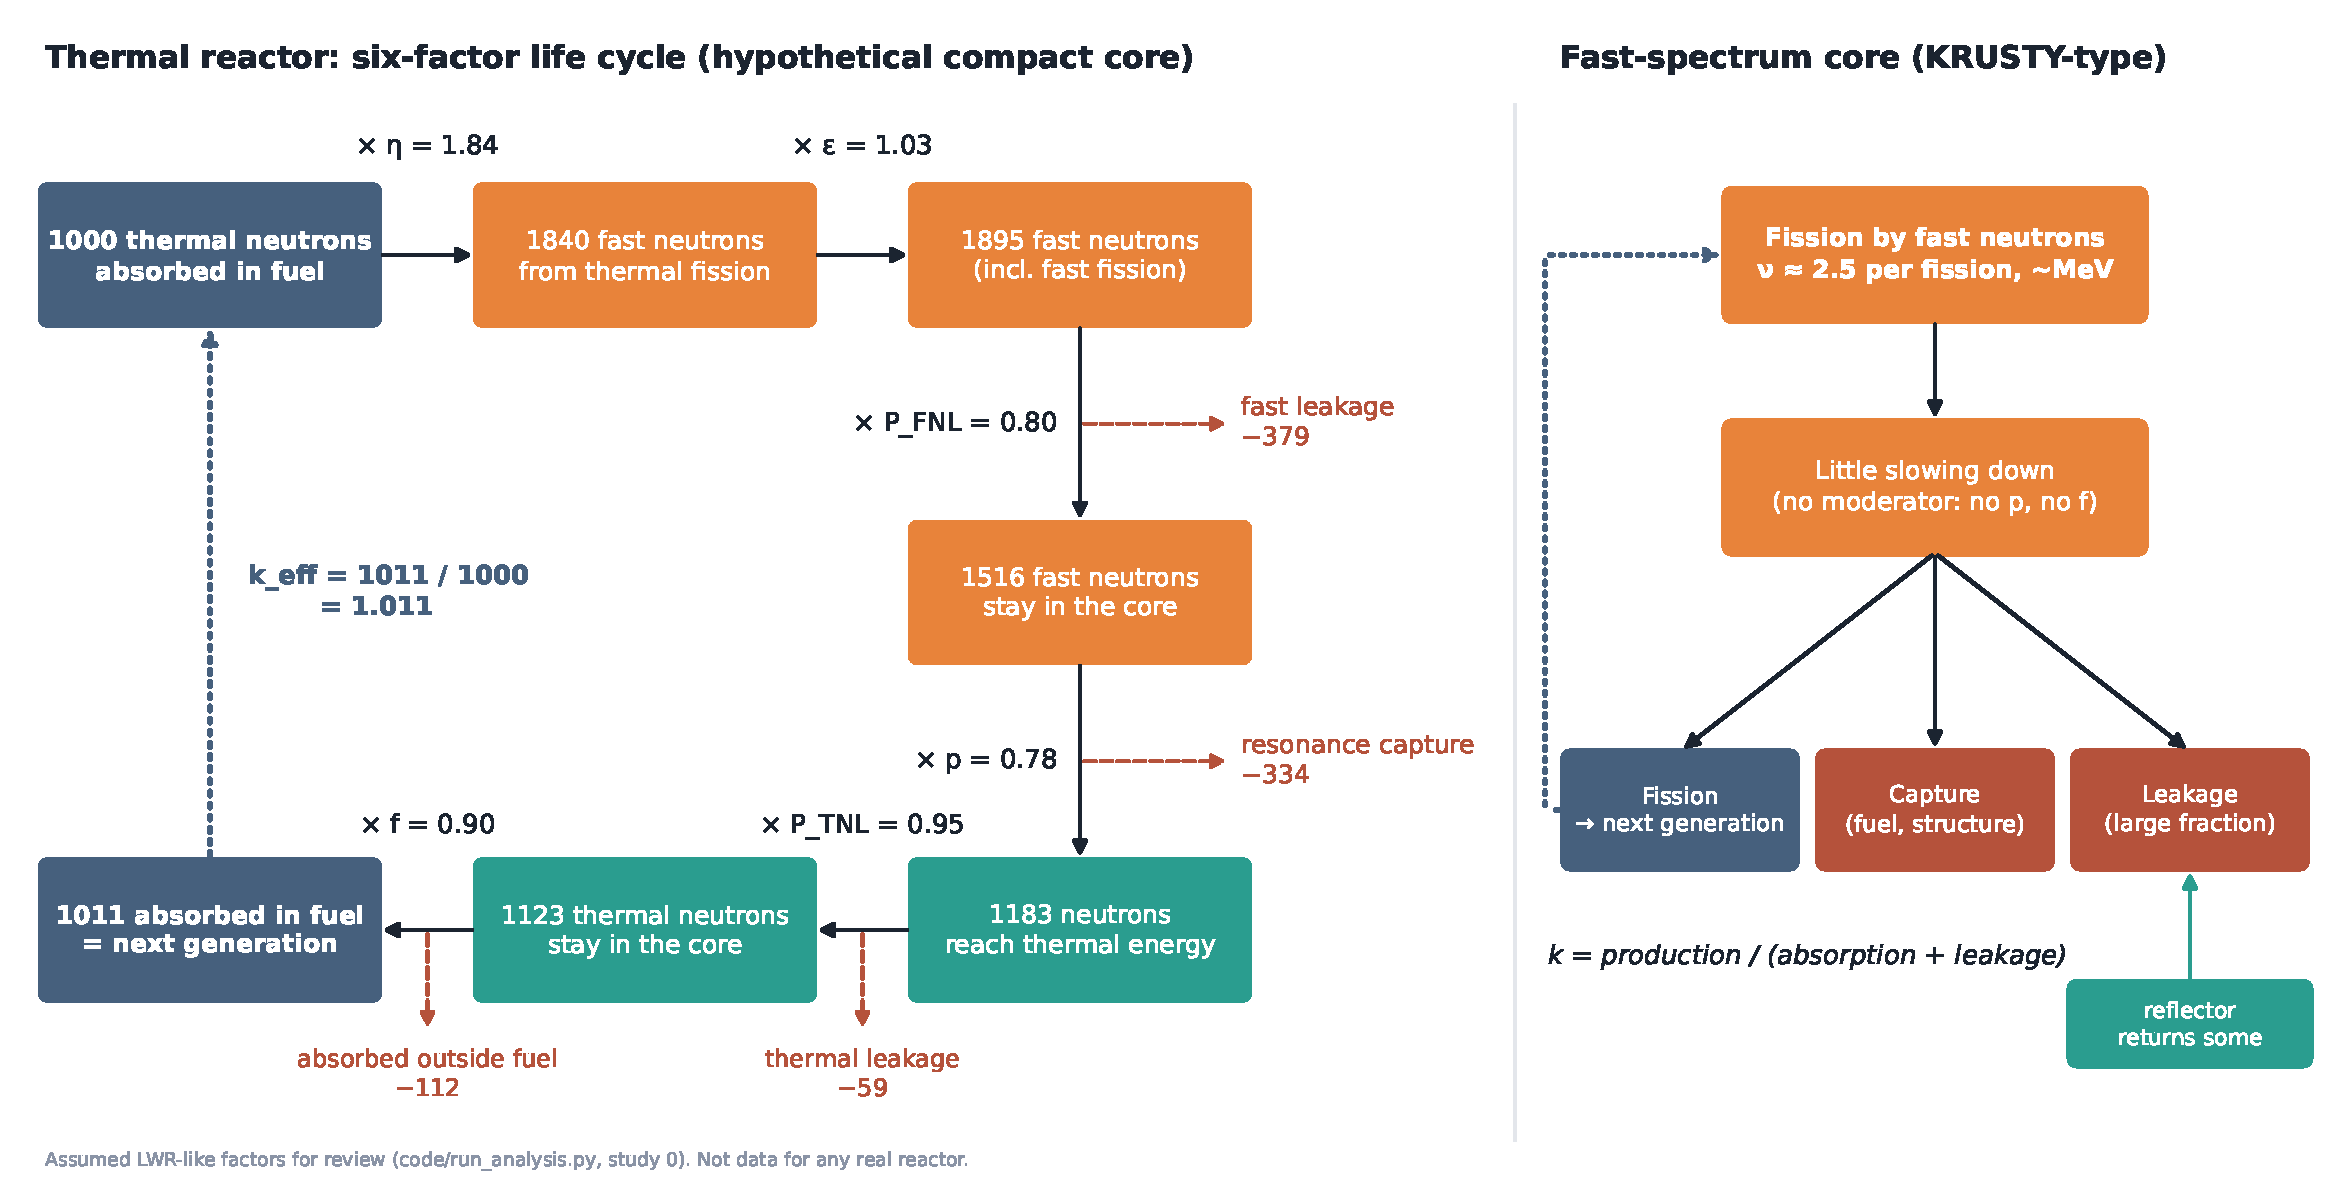
\includegraphics[width=\textwidth]{fig_life_cycle}
  \caption[Classical thermal life cycle versus fast-spectrum cycle]{Left: six-factor ledger with assumed factors (review only). Right: in a fast core the moderation, resonance-escape and thermal-utilization steps disappear and leakage dominates.}
  \label{fig:lifecycle}
\end{figure}

% =====================================================================
\section{Generalized Neutron Balance and the k-Eigenvalue Problem}
\label{sec:eigen}

\subsection{Transport formulation}
For angular flux $\psi(\mathbf{r},\boldsymbol{\Omega},E)$ in a source-free multiplying system, the steady transport equation with fission source divided by an eigenvalue $k$ is \citep{BellGlasstone1970,Duderstadt1976}
\begin{equation}
  \boldsymbol{\Omega}\cdot\nabla\psi + \Sigma_t\psi
  = \int_0^\infty\!\!\int_{4\pi}\Sigma_s(E'\!\to\!E,\boldsymbol{\Omega}'\!\cdot\!\boldsymbol{\Omega})\,\psi'\,d\Omega'\,dE'
  + \frac{\chi(E)}{4\pi k}\int_0^\infty \nu\Sigma_f(E')\,\phi(\mathbf{r},E')\,dE' ,
  \label{eq:transport}
\end{equation}
with a vacuum condition $\psi=0$ for incoming directions on the outer surface. In operator form, $\mathcal{L}\psi = k^{-1}\mathcal{F}\psi$, where $\mathcal{L}$ contains streaming, collisions and scattering and $\mathcal{F}$ the fission production. A physically meaningful (non-negative) solution exists only for the dominant eigenvalue, which is $\keff$. Integrating Eq.~\eqref{eq:transport} over all space, direction and energy gives Eq.~\eqref{eq:balance} exactly, with leakage as the net outward current through the surface.

\subsection{Multigroup form and why the six-factor formula is a special case}
Discretizing energy into $G$ groups gives coupled group equations whose fission sources share the single eigenvalue $k$. Each group has its own leakage, absorption and scattering to other groups. The six-factor formula follows only when there are two groups, all fissions are thermal except a correction ($\varepsilon$), the slowing-down and thermal problems are separable, and leakage of each group is represented by one non-leakage factor at a common buckling. In a fast core most fissions occur at \SIrange{0.1}{2}{MeV}, there is no thermal population to utilize, and energy-dependent leakage couples directly to the spectrum (Section~\ref{sec:spectral}). Equation~\eqref{eq:sixfactor} is therefore not wrong in principle. It is the wrong factorization for these systems.

\subsection{Power iteration}
The eigenvalue problem is solved by power iteration: starting from a guess $S^{(0)}$ of the fission source, $\psi^{(n+1)} = \mathcal{L}^{-1}S^{(n)}$, $S^{(n+1)} = \mathcal{F}\psi^{(n+1)}$, and $k^{(n+1)} = \int S^{(n+1)}/\int S^{(n)}$. The error decays with the dominance ratio, so the first iterations (``inactive'' generations in Monte Carlo) are discarded until the source shape has converged. Figure~\ref{fig:poweriter} shows this for the solver described in Section~\ref{sec:methods}.

\begin{figure}[ht]
  \centering
  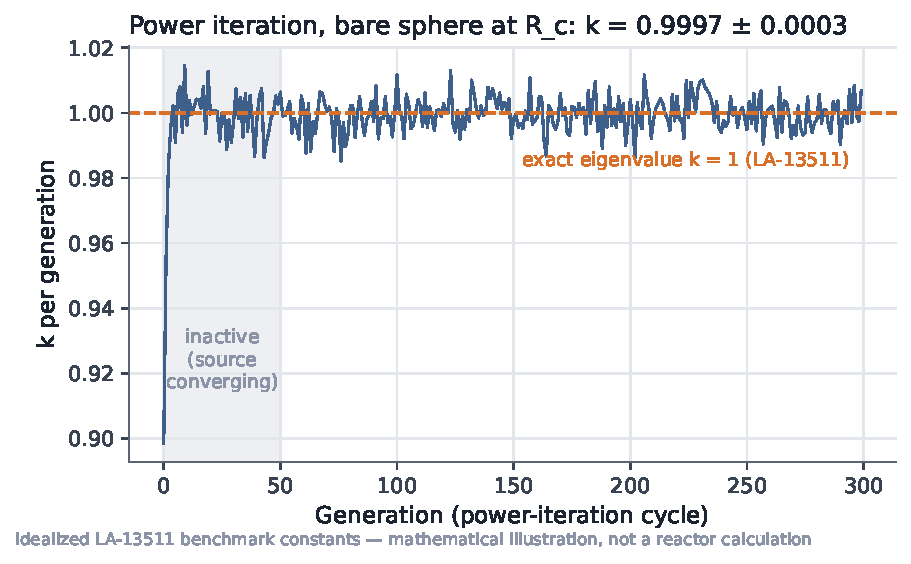
\includegraphics[width=0.72\textwidth]{fig_power_iteration}
  \caption[Monte Carlo power iteration]{Monte Carlo power iteration for the bare benchmark sphere Ua-1-0-SP: 50 inactive and 250 active generations of 40{,}000 neutrons. Mean $k = 0.99968 \pm 0.00033$; exact value 1.}
  \label{fig:poweriter}
\end{figure}

% =====================================================================
\section{One-Group Diffusion: Derivation and Validity}
\label{sec:diffusion}

\subsection{Derivation}
Integrating Eq.~\eqref{eq:transport} over direction and energy gives the one-group balance
\begin{equation}
  \nabla\cdot\mathbf{J} + \Sig{a}\phi = \frac{1}{k}\nu\Sig{f}\phi .
  \label{eq:onegroupbal}
\end{equation}
Closing it requires a relation between $\mathbf{J}$ and $\phi$. Expanding $\psi$ to first order in direction ($P_1$), $\psi \approx (\phi + 3\boldsymbol{\Omega}\cdot\mathbf{J})/4\pi$, and taking the first angular moment of the transport equation with isotropic sources gives Fick's law (Appendix~\ref{app:p1})
\begin{equation}
  \mathbf{J} = -D\nabla\phi, \qquad D = \frac{1}{3\Sig{tr}},\qquad \Sig{tr} = \Sigma_t - \bar\mu_0\Sigma_s .
\end{equation}
Substitution yields $D\nabla^2\phi - \Sig{a}\phi + k^{-1}\nu\Sig{f}\phi = 0$, or $\nabla^2\phi + B_m^2\phi = 0$ with material buckling $B_m^2 = (\nu\Sig{f}/k - \Sig{a})/D$. For a bare sphere the fundamental mode is $\phi \propto \sin(Br)/r$. Requiring $\phi$ to vanish at the extrapolated radius $R_e = R + d$, with $d \approx 0.7104\,\ltr$ from the Milne problem \citep{Duderstadt1976}, gives the geometric buckling $B_g^2 = (\pi/R_e)^2$. Setting $B_m^2 = B_g^2$:
\begin{equation}
  \keff = \frac{\kinf}{1 + L^2B_g^2}, \qquad \PNL = \frac{1}{1+L^2B_g^2}, \qquad L^2 = \frac{D}{\Sig{a}} .
  \label{eq:keffdiff}
\end{equation}
$L^2B_g^2$ is the ratio of leakage to absorption, and in one group with isotropic scattering $\keff = \kinf\PNL$ holds exactly, also in transport. This makes the transport leakage tally a direct test of what diffusion approximates.

\subsection{Validity}
Fick's law requires
\begin{enumerate*}[label=(\roman*)]
  \item a flux that varies slowly over a transport mean free path,
  \item weak absorption relative to scattering, and
  \item distance from boundaries, sources and strong absorbers
\end{enumerate*}
\citep{Duderstadt1976,Stacey2018}. A compact fast core is only 2--3 $\ltr$ in radius, so most neutrons are within a mean free path or two of a vacuum or a reflector interface, where the angular flux is strongly outward-directed. The extrapolation distance itself is a transport correction grafted onto diffusion. The following sections measure the consequences.

% =====================================================================
\section{Methods: Benchmark Data, Monte Carlo Solver and Verification}
\label{sec:methods}

\subsection{Benchmark cross sections}
All cross sections are taken from the LA-13511 analytic benchmark set \citep{Sood1999,Sood2003}, which provides idealized one- and two-group constants with exact transport critical dimensions. LA-13511 states that these constants are for code verification, not for predicting experiments. They were chosen because nothing is tuned and every answer is known. Table~\ref{tab:xs} lists the data. The one-group U-235 sets differ only in $\nu$. Sets b--d are used with water-like ($c = 0.90$) reflectors of 1, 2 and 3 mean free paths around a \SI{6.12745}{cm} core, each configuration being exactly critical. The two-group U-235 set has a fast fission spectrum fraction $\chi_\mathrm{fast} = 0.575$. The slow value is illegible in the available scan, and $\chi_\mathrm{slow} = 0.425$ was taken from normalization and confirmed by reproducing the published $\kinf = 2.216349$ and flux ratio 0.474967 exactly.

\begin{table}[ht]
\centering
\caption[Benchmark cross sections]{LA-13511 constants used in this work (\si{cm^{-1}}; isotropic scattering).}
\label{tab:xs}
\small
\begin{tabular}{@{}lcccccc@{}}
\toprule
Material & $\nu$ & $\Sig{f}$ & $\Sigma_c$ & $\Sigma_s$ & $\Sigma_t$ & Use \\
\midrule
U-235 (a) & 2.70 & 0.065280 & 0.013056 & 0.248064 & 0.32640 & bare sphere, studies 2--3, 5 \\
U-235 (b, c, d) & 2.797101, 2.707308, 2.679198 & \multicolumn{4}{c}{as (a)} & reflected benchmarks \\
H$_2$O ($c=0.90$) & -- & -- & 0.032640 & 0.293760 & 0.32640 & reflector \\
\midrule
U-235 fast & 2.70 & 0.06192 & 0.00384 & 0.07824 (to fast), 0.0720 (to slow) & 0.2160 & two-group \\
U-235 slow & 2.50 & 0.06912 & 0.01344 & 0.26304 & 0.3456 & two-group \\
\bottomrule
\end{tabular}
\end{table}

\subsection{Monte Carlo solver}
\texttt{code/mc_transport.py} implements an analog multigroup Monte Carlo k-eigenvalue solver for concentric spherical shells (Appendix~\ref{app:mc}). Histories alternate free flights and collisions. Scattering samples the outgoing group from the transfer matrix and an isotropic direction. Absorption produces fission with probability $\Sig{f}/\Sig{a}$, banking $\lfloor\nu + \xi\rfloor$ sites with groups sampled from $\chi$. Crossing the outer surface is leakage. The bank is resampled to $N$ sites per generation (power iteration), and $k$ is estimated with the collision estimator $\sum\nu\Sig{f}/\Sigma_t$ per source neutron. Life-cycle tallies record leakage, capture and fission by region and group, fissions caused by neutrons that had entered a reflector, and radial flux and fission density. Production runs used 40{,}000 neutrons per generation, 50 inactive and 250 active generations, with 80{,}000 neutrons and 400 active generations for the feedback study. Uncertainties are one standard deviation from generation-to-generation variation (inter-generation correlation neglected).

\subsection{Verification}
Table~\ref{tab:verify} compares the solver with the five exact solutions. All agree with $k = 1$ within about $1\sigma$. The flux shape of the bare critical sphere also agrees with the published flux ratios (Figure~\ref{fig:flux}). The solver is therefore used as the transport reference for these idealized problems.

\begin{table}[ht]
\centering
\caption[Verification against exact transport solutions]{Verification against exact LA-13511 solutions (exact $k=1$ in every case) and one-group diffusion at the same configuration.}
\label{tab:verify}
\small
\begin{tabular}{@{}llccc@{}}
\toprule
Problem & Configuration & Monte Carlo $k$ & Diffusion $k$ & Diffusion error \\
\midrule
Ua-1-0-SP & bare sphere, $R = 7.428998$ cm & $0.99968 \pm 0.00033$ & 0.93964 & $-6.0\%$ \\
Ub-H2O(1)-1-0-SP & core 6.12745 cm + 1 mfp H$_2$O & $1.00015 \pm 0.00034$ & 0.88317 & $-11.7\%$ \\
Uc-H2O(2)-1-0-SP & core 6.12745 cm + 2 mfp H$_2$O & $0.99998 \pm 0.00032$ & 0.89344 & $-10.7\%$ \\
Ud-H2O(3)-1-0-SP & core 6.12745 cm + 3 mfp H$_2$O & $1.00012 \pm 0.00033$ & 0.89664 & $-10.3\%$ \\
U-2-0-SP & two-group bare sphere, $R = 7.909444$ cm & $1.00010 \pm 0.00034$ & 0.93714 (2-group) & $-6.3\%$ \\
\bottomrule
\end{tabular}
\end{table}

\begin{figure}[ht]
  \centering
  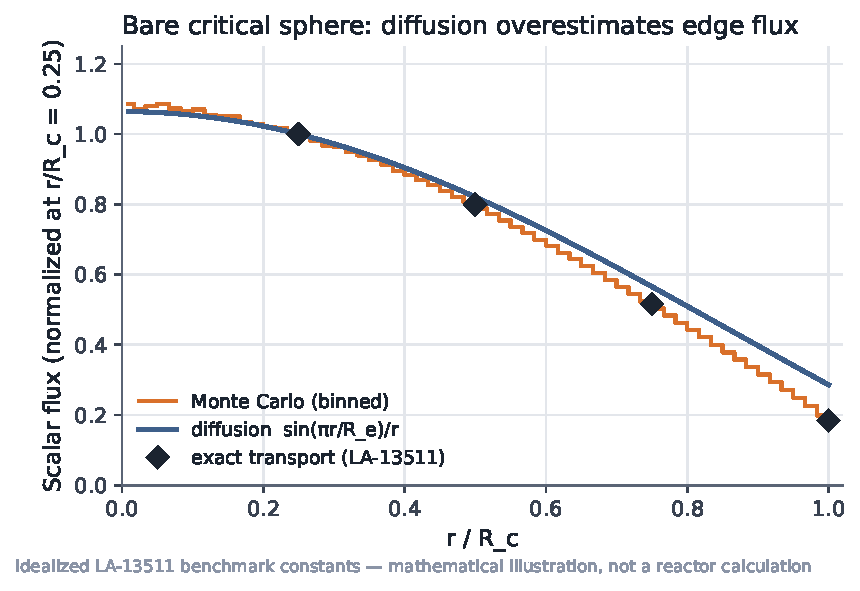
\includegraphics[width=0.66\textwidth]{fig_flux_shape}
  \caption[Flux shape: exact, Monte Carlo and diffusion]{Scalar flux in the bare critical sphere, normalized at $r/R_c = 0.25$. At the surface the exact value is 0.184, Monte Carlo 0.186 and diffusion 0.286.}
  \label{fig:flux}
\end{figure}

% =====================================================================
\section{Sensitivity of k\textsubscript{eff} to Size and Leakage}
\label{sec:sensitivity}

Table~\ref{tab:sens} and Figure~\ref{fig:sens} give $\keff$ and leakage of a bare U-235(a) sphere from 4 to \SI{14}{cm} ($\ltr = \SI{3.064}{cm}$, $\kinf = 2.25$). This is a mathematical illustration with idealized constants, not a reactor calculation.

\begin{table}[ht]
\centering
\caption[Sensitivity study results]{Bare-sphere sensitivity study: Monte Carlo transport vs one-group diffusion. Leakage is per source neutron; $\sigma_k \le 0.0005$.}
\label{tab:sens}
\small
\begin{tabular}{@{}rrcccccc@{}}
\toprule
$R$ [cm] & $R/\ltr$ & $k$ transport & $k$ diffusion & leakage (MC) & $1-\PNL$ (diff.) & diffusion error \\
\midrule
4.00 & 1.31 & 0.5707 & 0.5145 & 74.6\% & 77.1\% & $-9.84\%$ \\
5.00 & 1.63 & 0.7063 & 0.6432 & 68.6\% & 71.4\% & $-8.93\%$ \\
6.00 & 1.96 & 0.8341 & 0.7693 & 62.9\% & 65.8\% & $-7.77\%$ \\
7.00 & 2.28 & 0.9515 & 0.8900 & 57.7\% & 60.4\% & $-6.46\%$ \\
7.43 & 2.42 & 0.9998 & 0.9396 & 55.6\% & 58.2\% & $-6.01\%$ \\
8.00 & 2.61 & 1.0614 & 1.0034 & 52.8\% & 55.4\% & $-5.47\%$ \\
9.00 & 2.94 & 1.1607 & 1.1083 & 48.4\% & 50.7\% & $-4.51\%$ \\
10.00 & 3.26 & 1.2524 & 1.2046 & 44.3\% & 46.5\% & $-3.81\%$ \\
12.00 & 3.92 & 1.4086 & 1.3718 & 37.4\% & 39.0\% & $-2.62\%$ \\
14.00 & 4.57 & 1.5371 & 1.5083 & 31.7\% & 33.0\% & $-1.87\%$ \\
\bottomrule
\end{tabular}
\end{table}

\begin{figure}[ht]
  \centering
  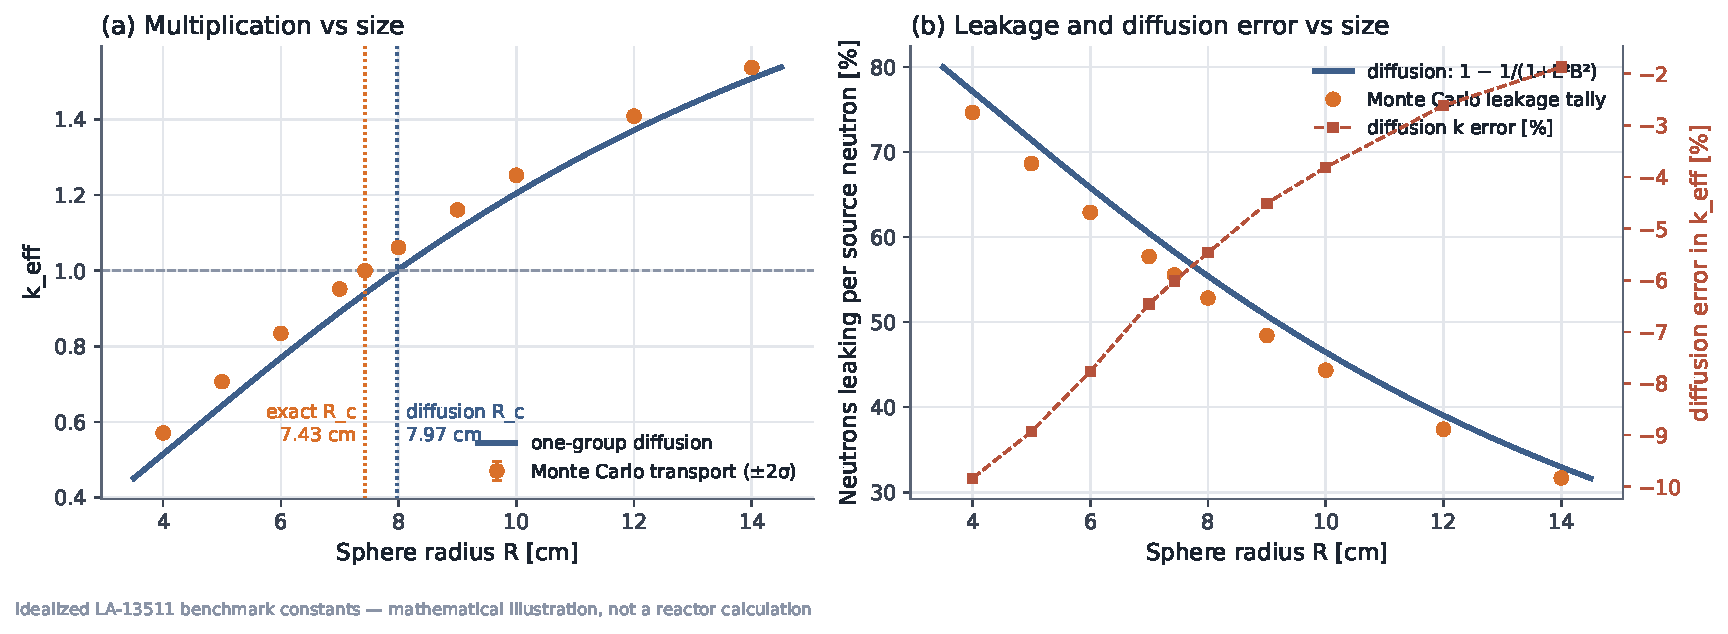
\includegraphics[width=\textwidth]{fig_sensitivity}
  \caption[k\textsubscript{eff}, leakage and diffusion error versus radius]{(a) $\keff$ versus radius. (b) Leakage per source neutron and diffusion error in $\keff$ (right axis).}
  \label{fig:sens}
\end{figure}

Three results stand out. First, between 32\% and 75\% of neutrons leak over this range, and 56\% at the exact critical radius: leakage is the largest loss term. Second, diffusion overestimates leakage at every size and therefore underestimates $\keff$. Its critical radius is \SI{7.969}{cm} against the exact \SI{7.429}{cm} ($+7.3\%$, or 24\% in critical mass). Third, the diffusion error falls monotonically with optical size, from 9.8\% at $1.3\,\ltr$ to 1.9\% at $4.6\,\ltr$. The governing variable is the size of the core in mean free paths, not its size in centimetres.

% =====================================================================
\section{Reflector Effects from Boundary Conditions}
\label{sec:reflector}

\subsection{Two-region diffusion}
A reflector is represented by its own diffusion equation and interface conditions, not by a multiplier on $\keff$. In a reflector of thickness $T$, $D_r\nabla^2\phi_r - \Sigma_{a,r}\phi_r = 0$ has the solution $\phi_r = C\sinh[\kappa(R + T_e - r)]/r$ with $\kappa = L_r^{-1}$ and $T_e = T + 0.7104\,\lambda_{\mathrm{tr},r}$. Continuity of flux and normal current at $r=R$ gives (Appendix~\ref{app:refl})
\begin{equation}
  D_c\bigl[BR\cot(BR) - 1\bigr] + D_r\bigl[\kappa R\coth(\kappa T_e) + 1\bigr] = 0,
  \qquad \keff = \frac{\nu\Sig{f}}{\Sig{a} + D_cB^2}.
  \label{eq:refl}
\end{equation}
Reflector savings is $\delta = R_{c,\mathrm{bare}} - R_{c,\mathrm{refl}}$. The familiar large-core estimate, $\delta \approx (D_c/D_r)\,L_r\tanh(T/L_r)$ \citep{Lamarsh2001}, assumes a nearly flat core flux at the interface.

\subsection{Results}
Using U-235(a) with the published water-like reflector ($L_r = \SI{5.59}{cm}$), the transport critical radius was found by secant iteration on Monte Carlo $\keff$ (Table~\ref{tab:refl}, Figure~\ref{fig:refl}).

\begin{table}[ht]
\centering
\caption[Reflector savings]{Critical core radius and reflector savings. Transport savings are relative to the exact bare radius \SI{7.428998}{cm}; diffusion savings are relative to the diffusion bare radius \SI{7.969}{cm}.}
\label{tab:refl}
\small
\begin{tabular}{@{}cccccc@{}}
\toprule
$T$ [cm] (mfp) & $R_c$ transport [cm] & $R_c$ diffusion [cm] & $\delta$ transport & $\delta$ diffusion & $\delta$ slab formula \\
\midrule
3.064 (1) & $6.406 \pm 0.003$ & 7.226 & 1.023 & 0.743 & 2.790 \\
6.127 (2) & $6.149 \pm 0.003$ & 6.911 & 1.280 & 1.058 & 4.468 \\
9.191 (3) & $6.073 \pm 0.002$ & 6.812 & 1.356 & 1.157 & 5.190 \\
\bottomrule
\end{tabular}
\end{table}

\begin{figure}[ht]
  \centering
  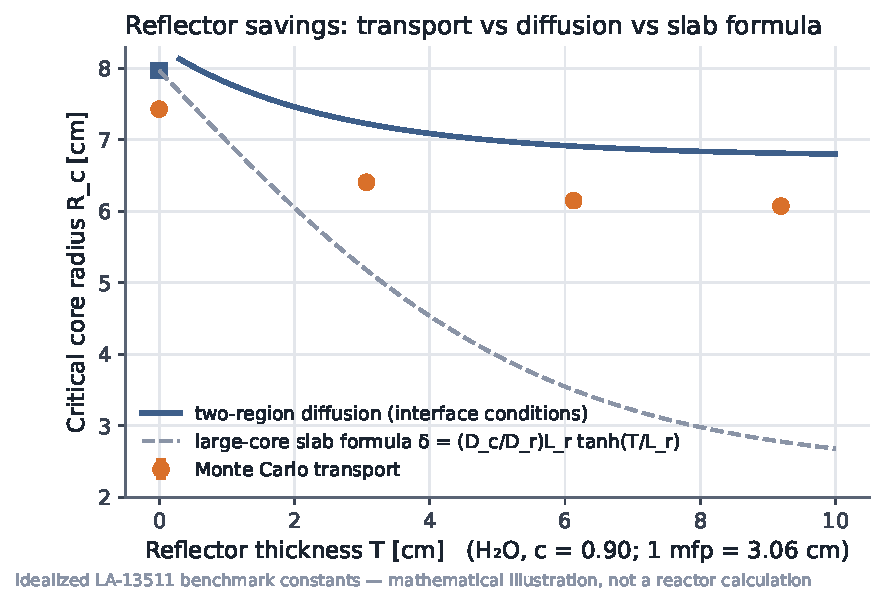
\includegraphics[width=0.68\textwidth]{fig_reflector_savings}
  \caption[Reflector savings: transport, diffusion and slab formula]{Critical core radius versus reflector thickness. The two-region diffusion curve starts at \SI{0.3}{cm} because its thin-reflector limit uses a different vacuum condition than the bare formula (square marker).}
  \label{fig:refl}
\end{figure}

Two-region diffusion underestimates the savings by 15--27\%, and its reflected critical radii are 12--13\% too large, a larger relative error than for the bare sphere. The slab formula overestimates the savings by a factor of 2.7--3.8, because the core flux near the interface is far from flat ($BL_r \approx 4.9$ here). The Monte Carlo life-cycle tallies give a physical picture of the reflector's role. In the three exact reflected benchmarks, 14.6\%, 17.8\% and 18.8\% of all fissions are caused by neutrons that had entered the reflector and returned. A reflector is a neutron source to the core edge, which in a real fast system means a softened spectrum and locally higher fission rates at the periphery (Section~\ref{sec:spectral}).

% =====================================================================
\section{Spectral Effects}
\label{sec:spectral}

The two-group U-235 benchmark separates fast and slow populations (Figure~\ref{fig:spectral}). In an infinite medium 32.2\% of the flux is in the fast group. In the critical sphere, 44.7\% of leaking neutrons and 37.7\% of fissions are fast. Leakage preferentially removes fast neutrons, which have the longer mean free path ($1/\Sigma_t = \SI{4.63}{cm}$ fast versus \SI{2.89}{cm} slow). As a result, the fast-to-slow flux ratio inside the finite core is about 0.65--0.68, against 0.475 in the infinite medium, and it rises further at the surface. The fundamental-mode diffusion spectrum at the critical buckling gives 0.677, consistent with the interior Monte Carlo values.

\begin{figure}[ht]
  \centering
  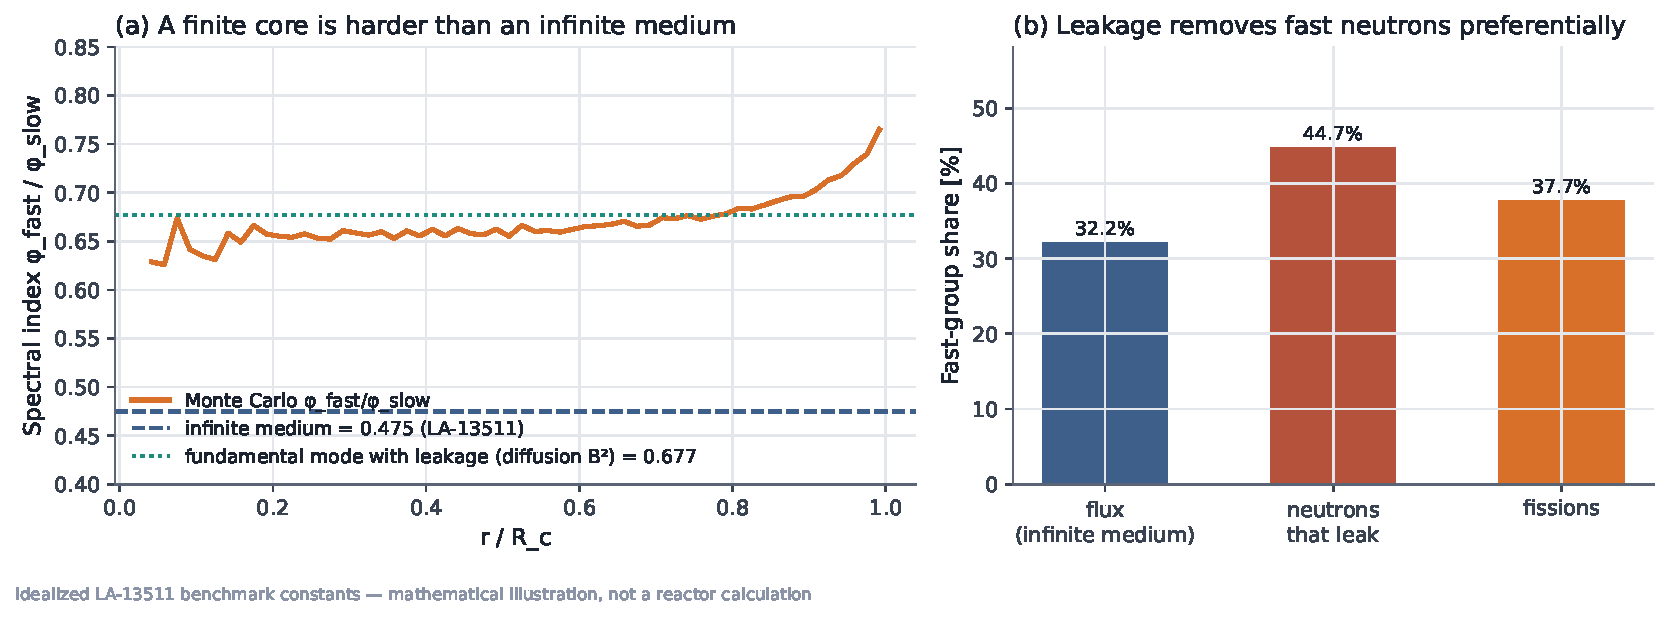
\includegraphics[width=\textwidth]{fig_spectral}
  \caption[Spectral effects of leakage]{(a) Fast-to-slow flux ratio versus radius in the critical two-group sphere. (b) Fast-group share of infinite-medium flux, of leaking neutrons and of fissions.}
  \label{fig:spectral}
\end{figure}

This matters whenever cross sections are collapsed. Collapsing the two-group set to one group with the infinite-medium spectrum gives a transport critical radius of $\SI{7.822 \pm 0.002}{cm}$, 1.1\% below the exact two-group value of \SI{7.909}{cm}. Weighting with the leakage-corrected (finite-buckling) spectrum reduces the error to 0.6\%. For comparison, two-group diffusion overpredicts the critical radius by 7.7\% (\SI{8.520}{cm}). In this idealized case the spectral-collapse error is roughly seven times smaller than the angular (diffusion) error. The ranking is specific to these constants, but it indicates the order of priorities: transport first, then energy resolution.

Real reflected fast cores add a spectral effect the two-group bare model cannot show. The KRUSTY design paper notes that fuel feedback is concentrated in a thin region around the perimeter of the fuel, due to moderated neutrons returning from the BeO reflector \citep{Poston2020Design}. Neutrons that slow down in a moderating reflector return with larger fission cross sections and peak the fission rate at the fuel edge. One-group or homogenized models miss this coupling of spectrum and geometry.

% =====================================================================
\section{KRUSTY: Reflector Worth and Reactivity Control}
\label{sec:krustyworth}

KRUSTY was a NASA--DOE nuclear ground test of a \SI{1}{kWe}-class Kilopower reactor. It was conducted in March 2018 at the National Criticality Experiments Research Center, Nevada National Security Site, on the COMET critical assembly machine \citep{Poston2020Results,Poston2020Design}. The core was an annulus of HEU (93.1 wt\% \textsuperscript{235}U) alloyed with 7.65 wt\% Mo, \SI{11}{cm} OD, \SI{4}{cm} ID and \SI{25}{cm} tall (\SI{32.2}{kg}). It was surrounded by BeO axial and radial reflectors, had a central B\textsubscript{4}C rod, and transported heat through eight sodium heat pipes \citep{Sanchez2020Component,Stolte2022,Poston2020Results}. Figure~\ref{fig:krusty} is a simplified schematic.

\begin{figure}[ht]
  \centering
  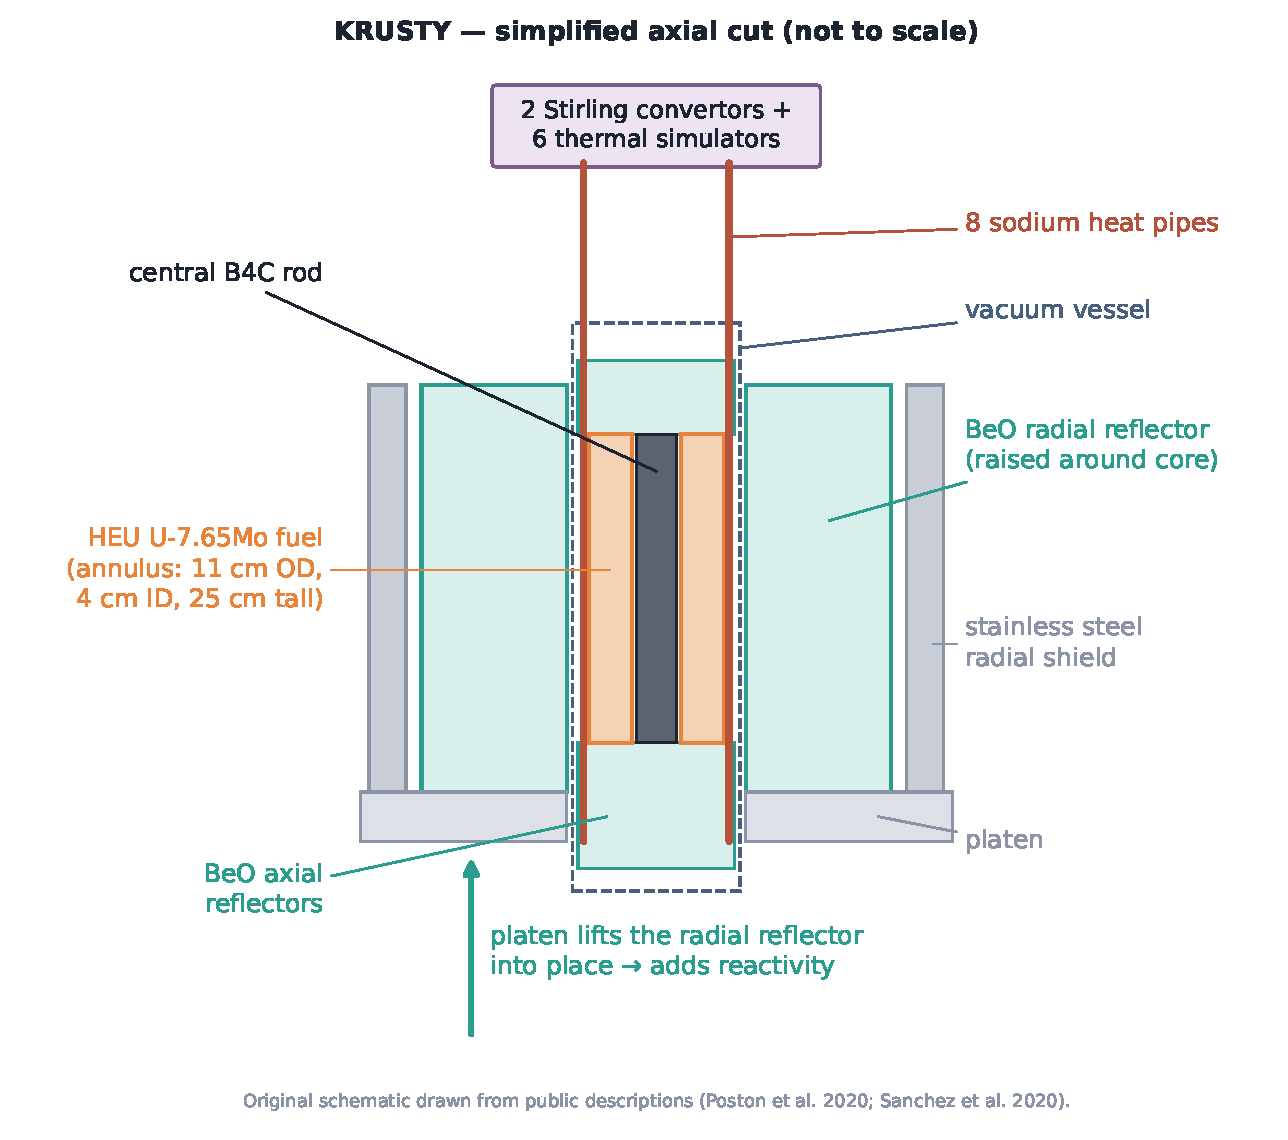
\includegraphics[width=0.6\textwidth]{fig_krusty_schematic}
  \caption[Simplified KRUSTY schematic]{Simplified axial cut of KRUSTY in its operating configuration, drawn from public descriptions \citep{Poston2020Design,Sanchez2020Component}. Not to scale.}
  \label{fig:krusty}
\end{figure}

Reactivity was controlled by lifting the radial BeO reflector on the COMET platen. The measured platen worth was about \SI{12.0}{\text{\textcent}/mm} at the start of the test and \SI{10.7}{\text{\textcent}/mm} later. The B\textsubscript{4}C rod near its expected critical position was worth about \SI{4}{\text{\textcent}/mm}, roughly one-third as sensitive \citep{Poston2020Results}. About \SI{1.42}{\$} was inserted to bring the fuel to \SI{800}{\celsius} \citep{Poston2020Results}. The design model gives a fuel temperature defect of \SI{-148.1}{\text{\textcent}} at \SI{1093}{K}, and a sum over all components of \SI{-146.4}{\text{\textcent}} (Table~\ref{tab:tableII}) \citep{Poston2020Design}. Reactivity is quoted with $\beta_\mathrm{eff} = 0.00688$ from MCNP \citep{Poston2020Design}.

Three points follow. First \obs, reflector motion, not absorber motion, was the operational control: a millimetre of reflector was worth about three millimetres of absorber rod. This is the experimental face of a leakage-dominated balance (Sections~\ref{sec:sensitivity}--\ref{sec:reflector}). Second \infr, the reactivity added by the platen to reach \SI{800}{\celsius} (142~\textcent) is comparable to the model's total temperature defect (146~\textcent). That is consistent with a picture in which reflector insertion offsets the fuel's negative feedback during heat-up. This is an inference from two published numbers, not a measured balance. Third \obs, the initial, unadjusted MCNP model predicted the first critical within 30~\textcent\ and each incremental configuration change within a few cents \citep{Poston2020Warm}. That is the fidelity continuous-energy transport delivers, against the 6--12\% $\keff$ errors of one-group diffusion in Table~\ref{tab:verify}.

% =====================================================================
\section{KRUSTY: Decomposition of Negative Reactivity Feedback}
\label{sec:feedback}

\subsection{Published decomposition}
The KRUSTY design paper attributes about 95\% of net reactor feedback to fuel heating. About 90\% of the fuel feedback comes from thermal expansion and about 10\% from changes in fuel cross sections \citep{Poston2020Design}. Doppler broadening falls in the latter category. With 93\% enriched fuel the \textsuperscript{238}U content is small, so a small Doppler contribution is physically expected \infr. Table~\ref{tab:tableII} and Figure~\ref{fig:krustyfb} reproduce the published component coefficients.

\begin{table}[ht]
\centering
\caption[KRUSTY component feedback (published)]{KRUSTY component reactivity feedback, reproduced from Poston et al., \emph{KRUSTY Reactor Design}, Table II \citep{Poston2020Design} (design-model values).}
\label{tab:tableII}
\small
\begin{tabular}{@{}lccc@{}}
\toprule
Component & Operating temperature [K] & Temperature defect [\textcent] & Average coefficient [\textcent/K] \\
\midrule
Fuel & 1093 & $-148.1$ & $-0.1844$ \\
Heat pipes & 1073 & $-1.2$ & $-0.0015$ \\
Ring clamp & 1068 & $-2.1$ & $-0.0027$ \\
Axial reflector & 473 & $-0.1$ & $-0.0005$ \\
Vacuum can & 393 & $+2.4$ & $+0.0233$ \\
Radial reflector & 343 & $+3.1$ & $+0.0585$ \\
Platen and shielding & 323 & $-0.4$ & $-0.0121$ \\
\bottomrule
\end{tabular}
\end{table}

\begin{figure}[ht]
  \centering
  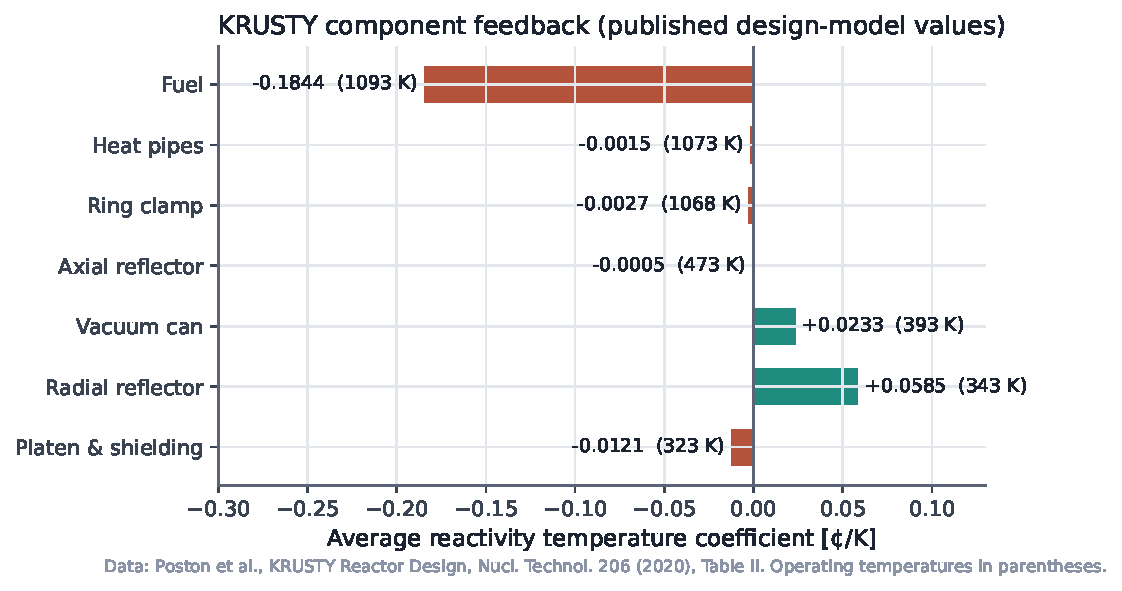
\includegraphics[width=0.7\textwidth]{fig_krusty_feedback}
  \caption[KRUSTY component feedback]{Published KRUSTY component temperature coefficients (Table~\ref{tab:tableII}).}
  \label{fig:krustyfb}
\end{figure}

Two components have positive coefficients at their test temperatures. For the vacuum can, the test-results paper explains that axial thermal expansion lowers the fuel relative to the radial reflector, the same effect as raising the platen \citep{Poston2020Results}. For the radial BeO reflector, expansion feedback (negative) and cross-section feedback (positive) balance near \SI{600}{K}. The authors note that a flight system would have much less positive BeO feedback and no comparable relative motion between fuel and reflector \citep{Poston2020Results}. The design paper also states that heating the radial reflector provides significant negative feedback, which the short test window did not allow \citep{Poston2020Design}. These statements are consistent with the positive coefficient at \SI{343}{K} if the reflector's net coefficient changes sign above about \SI{600}{K} \infr. Measured system behaviour agrees in kind: a fuel temperature feedback coefficient of about \SI{0.2}{\text{\textcent}/\celsius} near \SI{800}{\celsius} (negative) and passive load following \obs\ \citep{Poston2020Results}.

\subsection{First-principles estimate of expansion feedback}
For uniform isotropic thermal strain $\varepsilon = \alpha\Delta T$, number densities scale as $(1+\varepsilon)^{-3}$ and lengths as $(1+\varepsilon)$. In one group, $\keff$ of a bare homogeneous sphere depends only on its optical radius $\Sigma_tR \propto (1+\varepsilon)^{-2}$, so expansion always increases leakage. The reactivity coefficient follows as
\begin{equation}
  \alpha_T \approx \frac{1}{\beta_\mathrm{eff}}\,\frac{d\ln\keff}{d\varepsilon}\,\alpha .
  \label{eq:alphaT}
\end{equation}
Monte Carlo runs at $\varepsilon = \pm 0.01$ (Table~\ref{tab:fb}) give $d\ln\keff/d\varepsilon = -1.654 \pm 0.013$ for the bare critical sphere ($-1.802$ in diffusion). They give $-1.455 \pm 0.013$ when only the core of the reflected benchmark Ub-H2O(1) expands, and $-0.290 \pm 0.014$ when only its reflector expands. With $\alpha = \SI{17.2e-6}{K^{-1}}$, the mean coefficient of U-10Mo from room temperature to \SI{800}{\celsius} \citep{Burkes2010}, used as a proxy for U-7.65Mo, and $\beta_\mathrm{eff} = 0.00688$ \citep{Poston2020Design}, Eq.~\eqref{eq:alphaT} gives $-0.413 \pm 0.003$ (bare) and $-0.364 \pm 0.003$~\textcent/K (reflected core). The uncertainties are statistical only.

\begin{table}[ht]
\centering
\caption[Expansion feedback estimates]{Reactivity response to uniform thermal expansion (idealized benchmark spheres) compared with published KRUSTY values.}
\label{tab:fb}
\small
\begin{tabular}{@{}lcc@{}}
\toprule
Case & $d\ln\keff/d\varepsilon$ & Coefficient [\textcent/K] \\
\midrule
Bare sphere, core expands (MC) \calc & $-1.654 \pm 0.013$ & $-0.413$ \\
Bare sphere, core expands (diffusion) \calc & $-1.802$ & $-0.450$ \\
Reflected, core only expands (MC) \calc & $-1.455 \pm 0.013$ & $-0.364$ \\
Reflected, reflector only expands (MC) \calc & $-0.290 \pm 0.014$ & -- \\
\midrule
KRUSTY fuel, expansion share (90\% of $-0.1844$) & -- & $-0.166$ \\
KRUSTY fuel, total (design model) & -- & $-0.1844$ \\
KRUSTY measured, near \SI{800}{\celsius} & -- & $\approx -0.2$ \\
\bottomrule
\end{tabular}
\end{table}

\begin{figure}[ht]
  \centering
  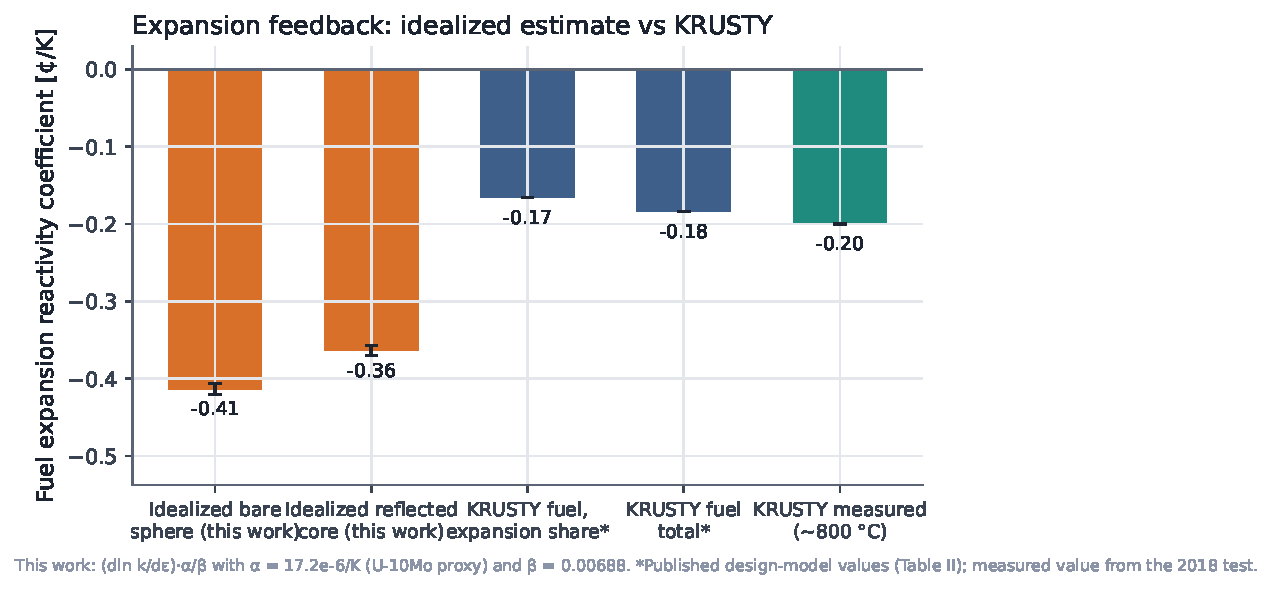
\includegraphics[width=0.7\textwidth]{fig_feedback_compare}
  \caption[Expansion feedback: estimate versus KRUSTY]{Idealized expansion-feedback estimates from this work compared with published KRUSTY design-model and measured values.}
  \label{fig:fbcompare}
\end{figure}

The estimate has the correct sign and order of magnitude and is about twice the KRUSTY expansion share. The difference is expected and is not apportioned here. The model is a homogeneous sphere with benchmark constants, not an annular cylinder with heat pipes and a thick BeO reflector; it expands isotropically and without constraint; it uses a proxy expansion coefficient; and it omits all cross-section temperature effects. Two qualitative results are robust within the model. Reflection reduces the core's expansion sensitivity (by 12\% here). Expanding a non-moderating reflector also gives negative feedback, which KRUSTY's BeO offsets through cross-section effects at low temperature.

% =====================================================================
\section{Limitations of Diffusion Theory and the Role of Continuous-Energy Monte Carlo}
\label{sec:limits}

The calculations above quantify diffusion's failure modes for compact systems:
\begin{enumerate*}[label=(\roman*)]
  \item boundary error: the flux at a vacuum surface is overestimated by more than 50\% (Figure~\ref{fig:flux});
  \item size error: 2--10\% in $\keff$ for radii of 1.3--4.6 $\ltr$;
  \item interface error: 10--12\% in thin-reflector configurations; and
  \item reflector-savings formulas that assume flat fluxes fail by factors of 3--4.
\end{enumerate*}
Real space reactors add heterogeneity (annular fuel, heat-pipe channels, gaps, an internal absorber), anisotropic scattering, resonance and thermal-scattering physics in reflectors such as BeO, and temperature-dependent cross sections. Multigroup diffusion with transport-corrected constants reduces some of these errors, and deterministic transport (discrete ordinates) removes the angular approximation. Continuous-energy Monte Carlo with evaluated data, such as OpenMC \citep{Romano2015}, represents the geometry and energy dependence directly and can compute reflector worth, component temperature coefficients (by perturbing geometry and Doppler-broadened data) and fission-rate distributions in one consistent model.

High fidelity is not the same as validation. The KRUSTY component-critical benchmark evaluation \citep{Stolte2022} supplies measured configurations with quantified uncertainties against which any such model must first be tested. The repository therefore includes an OpenMC input set (\texttt{openmc/}) with a planned sequence: multigroup reproduction of the LA-13511 problems as an independent check of the in-house solver, a continuous-energy bare HEU sphere (Godiva, HEU-MET-FAST-001; modeled radius about \SI{8.74}{cm} \citep{Trkov2020}), then a KRUSTY component-critical model. \emph{These inputs have not been run, and no OpenMC results are reported.}

% =====================================================================
\section{Findings and Implications for Neutron Economy}
\label{sec:findings}

\paragraph{Calculated results (this work; idealized benchmark constants).}
\begin{enumerate}[label=C\arabic*.]
  \item The in-house Monte Carlo solver reproduces five exact transport solutions within about $1\sigma$ ($\sigma \approx 0.0003$).
  \item One-group diffusion underpredicts $\keff$ by 6\% (bare) and 10--12\% (reflected) at exactly critical compact configurations, and overpredicts the bare critical radius by 7.3\%. The error decreases from 9.8\% to 1.9\% as the radius increases from 1.3 to 4.6 $\ltr$.
  \item Leakage is 32--75\% of all neutron losses over the sizes studied. Transport reflector savings are 1.0--1.4~cm, the slab formula overestimates them 2.7--3.8 times, and 15--19\% of fissions in reflected benchmarks are caused by reflector-returned neutrons.
  \item Leakage preferentially removes fast neutrons (44.7\% of leakage versus 32.2\% of infinite-medium flux). One-group collapse error is about 1\% (0.6\% with a leakage-weighted spectrum), several times smaller than diffusion error here.
  \item Uniform expansion gives $d\ln\keff/d\varepsilon \approx -1.5$ to $-1.7$. With a U-Mo proxy expansion coefficient this corresponds to $-0.36$ to $-0.41$~\textcent/K.
\end{enumerate}

\paragraph{Established experimental observations (KRUSTY, published).}
\begin{enumerate}[label=E\arabic*.]
  \item Reactivity was controlled by raising the BeO radial reflector, with a platen worth of 10.7--12.0~\textcent/mm, about three times the sensitivity of the B\textsubscript{4}C rod.
  \item About 1.42~\$ was inserted to reach \SI{800}{\celsius}. The measured fuel temperature feedback was about $-0.2$~\textcent/\si{\celsius}, and the reactor load-followed passively.
  \item The unadjusted MCNP model predicted the first critical within 30~\textcent\ and incremental changes within a few cents.
\end{enumerate}
\emph{Published design-model results} (not measurements) supply the component decomposition: fuel $\approx$95\% of net feedback; within the fuel, 90\% expansion and 10\% cross sections; positive coefficients for the vacuum can and radial reflector at test temperatures.

\paragraph{Engineering inferences.}
\begin{enumerate}[label=I\arabic*.]
  \item In compact fast cores, criticality is predominantly a property of geometry and leakage. Small dimensional changes (expansion, gaps, reflector position) are reactivity changes of the order of dollars.
  \item The sign and size of temperature feedback depend on which component heats and how components move relative to each other, so feedback must be resolved by component and temperature, not assumed from fuel Doppler.
  \item Because diffusion errors of 5--12\% in $\keff$ correspond to many dollars of reactivity, one-group or homogenized models can guide intuition but not design. Conclusions require validated transport.
\end{enumerate}

\paragraph{Implications for neutron economy and criticality.}
In a large thermal reactor neutron economy is mostly about where absorptions occur (the factors $p$ and $f$). In a compact fast core it is mostly about how many neutrons leave and how many are sent back. This changes how criticality should be read. Excess reactivity, control worth, shutdown margin and feedback all derive from the same leakage term. Any uncertainty in modeling leakage, from boundary treatment, reflector representation or spectrum, propagates into all of them at once. None of the simplified models here is a design tool. Their value is to show where the errors are and how large they are.

% =====================================================================
\section{Conclusions and Future Work}
\label{sec:conclusions}

\begin{enumerate}
  \item The six-factor formula is a special, separable case of the k-eigenvalue problem. It remains the right conceptual foundation, but it is the wrong factorization for compact fast-spectrum reactors.
  \item Leakage, reflection and spectrum are coupled. In verified calculations on compact benchmark systems, one-group diffusion misses this coupling by 5--12\% in $\keff$, and simple reflector-savings formulas fail by factors of 3--4.
  \item KRUSTY shows the physics experimentally: reflector position was the control, and fuel thermal expansion through increased leakage provided most of the stabilizing feedback. Published component data show feedback signs that depend on temperature and configuration.
\end{enumerate}

\paragraph{Future work.}
\begin{enumerate*}[label=(\roman*)]
  \item run the provided OpenMC multigroup inputs as an independent check;
  \item build and validate a continuous-energy KRUSTY component-critical model against the published benchmark;
  \item compute reflector worth versus platen height and component temperature coefficients with that model;
  \item extend the expansion analysis to anisotropic, constrained expansion in cylindrical geometry; and
  \item examine how HALEU fuel, as in current NASA plans, changes leakage fractions and the Doppler share of feedback.
\end{enumerate*}

% =====================================================================
\bibliographystyle{unsrtnat}
\bibliography{references}

% =====================================================================
\appendix
\newpage
\section{Mathematical Derivations}
\label{app:derivations}

\subsection{\texorpdfstring{$P_1$ approximation and Fick's law}{P1 approximation and Fick's law}}
\label{app:p1}
Write the one-group angular flux as $\psi(\mathbf r,\boldsymbol\Omega) \approx \frac{1}{4\pi}\phi + \frac{3}{4\pi}\boldsymbol\Omega\cdot\mathbf J$, which reproduces $\phi=\int\psi\,d\Omega$ and $\mathbf J=\int\boldsymbol\Omega\psi\,d\Omega$. Multiply the transport equation by $\boldsymbol\Omega$ and integrate over angle. With $\int\Omega_i\Omega_j\,d\Omega = \frac{4\pi}{3}\delta_{ij}$, isotropic fission and a linearly anisotropic scattering kernel with mean cosine $\bar\mu_0$:
\[
\tfrac{1}{3}\nabla\phi + \Sigma_t\mathbf J = \bar\mu_0\Sigma_s\mathbf J
\quad\Rightarrow\quad
\mathbf J = -\frac{1}{3(\Sigma_t-\bar\mu_0\Sigma_s)}\nabla\phi = -D\nabla\phi .
\]
The truncation is accurate when the angular flux is nearly isotropic, which fails within a few mean free paths of a vacuum boundary.

\subsection{Bare sphere and the non-leakage probability}
With $u = r\phi$, $\nabla^2\phi + B^2\phi = 0$ becomes $u'' + B^2u = 0$, so $\phi = A\sin(Br)/r$ (finite at the origin). The condition $\phi(R_e)=0$ gives $B = \pi/R_e$. Integrating the diffusion equation over the volume, total leakage $= DB^2\int\phi\,dV$ and absorption $=\Sig{a}\int\phi\,dV$, so $\PNL = 1/(1+L^2B^2)$.

\subsection{Reflected sphere}
\label{app:refl}
In the reflector, $u'' - \kappa^2u = 0$ with $u = r\phi_r$ and the condition $\phi_r(R+T_e)=0$ give $\phi_r = C\sinh[\kappa(R+T_e-r)]/r$. The logarithmic derivatives at $r=R$ are $\phi_c'/\phi_c = B\cot(BR) - 1/R$ and $\phi_r'/\phi_r = -\kappa\coth(\kappa T_e) - 1/R$. Equating $D_c\phi_c'$ and $D_r\phi_r'$ with $\phi_c=\phi_r$ and multiplying by $R$ gives Eq.~\eqref{eq:refl}. The root $B\in(0,\pi/R)$ is found by Brent's method.

\subsection{Multigroup diffusion for a bare sphere}
With group buckling $B_g^2 = [\pi/(R + 0.7104/\Sigma_{t,g})]^2$, the group equations are $(D_gB_g^2 + \Sigma_{t,g})\phi_g - \sum_{g'}\Sigma_{s,g'\to g}\phi_{g'} = k^{-1}\chi_g\sum_{g'}\nu\Sigma_{f,g'}\phi_{g'}$. $\keff$ is the largest eigenvalue of $\mathbf M^{-1}\mathbf F$. The normalized eigenvector is the leakage-weighted spectrum used for the second collapse in Section~\ref{sec:spectral}.

\subsection{Expansion scaling}
For strain $\varepsilon$, $N \to N(1+\varepsilon)^{-3}$ and $R \to R(1+\varepsilon)$. In one group with all macroscopic cross sections proportional to $N$, $\keff$ of a bare sphere depends only on $\Sigma_tR \propto (1+\varepsilon)^{-2}$. Hence $d\ln\keff/d\varepsilon = -2\,d\ln\keff/d\ln(\Sigma_tR)$, and the bare critical radius scales exactly as $1/N$.

% =====================================================================
\section{Monte Carlo Algorithm and Statistics}
\label{app:mc}
Each history starts at a fission site with a group sampled from $\chi$ and an isotropic direction. The distance to collision is $-\ln\xi/\Sigma_t$; the distance to the next spherical surface is computed analytically. If the collision is nearer, the neutron collides: scattering with probability $\Sigma_s/\Sigma_t$ (outgoing group from the cumulative transfer row), otherwise absorption, which is fission with probability $\Sig{f}/\Sig{a}$, banking $\lfloor\nu+\xi\rfloor$ sites. Otherwise the neutron crosses the surface. Leaving the outermost surface terminates the history as leakage, and entering a region flagged as reflector sets a ``visited reflector'' flag. Each generation the bank is resampled uniformly to $N$ sites. The per-generation collision estimator $k = N^{-1}\sum_{\text{collisions}}\nu\Sig{f}/\Sigma_t$ is averaged over active generations, and its standard error is the sample standard deviation divided by $\sqrt{n_\mathrm{active}}$. Flux is tallied with the collision estimator $1/\Sigma_t$ in 60 equal-width radial shells divided by shell volume. At the outer surface it is extrapolated linearly from the last two shells. Critical radii are found by secant iteration followed by a linear fit through the three points closest to $k=1$. Their uncertainty is $\sigma_k/|dk/dR|$. Runtime for the full study is about 4--5 minutes on a laptop (numba-compiled).

% =====================================================================
\section{Code and Reproducibility}
\label{app:code}
Python 3.9+ with \texttt{numpy}, \texttt{scipy}, \texttt{numba} and \texttt{matplotlib}. From the repository root:
\begin{verbatim}
pip install -r code/requirements.txt
python code/benchmarks.py        # checks the published constants (k_inf, c, flux ratio)
python code/run_analysis.py      # all studies -> results/analysis_results.json, .txt
python code/make_figures.py      # report figures (add --dark for slide versions)
python code/make_diagrams.py     # conceptual diagrams
\end{verbatim}
Every number in this report appears in \texttt{results/analysis\_output.txt}. The core solver is listed below.

\lstinputlisting[caption={\texttt{code/mc\_transport.py}}]{../code/mc_transport.py}
\lstinputlisting[caption={\texttt{code/diffusion.py}}]{../code/diffusion.py}

% =====================================================================
\section{OpenMC Input (Not Yet Run)}
\label{app:openmc}
\texttt{openmc/mg\_benchmarks.py} writes the Table~\ref{tab:xs} constants to OpenMC multigroup libraries and builds the five verification problems with vacuum boundaries. The expected result is $k = 1$ within statistics. The continuous-energy steps (Godiva, then the KRUSTY component-critical configuration from Stolte et al.\ \citep{Stolte2022}) are described in \texttt{openmc/README.md}. Their compositions are to be taken from the benchmark documents themselves and are intentionally not typed into the repository.

\end{document}
